\section{Kernels}
\smallskip \hrule height 2pt \smallskip
If the data is not linearly separable and/or you want a wiggly boundary, use kernels. 

Can use for things you can't handle with slack variables.  % wk 8 audio

Start w/ original feature space, use polynomial of degree d, and get a higher dimensional space
    then do a linear classifier in this space.   % wk 8 audio
\hfill \\  \hfill \\

Can give you nonlinear boundaries (good) but the feature space can get really large really quickly. 

Example mapping of data that is not linearly separable to a separable higher dimension space: \hfill \\
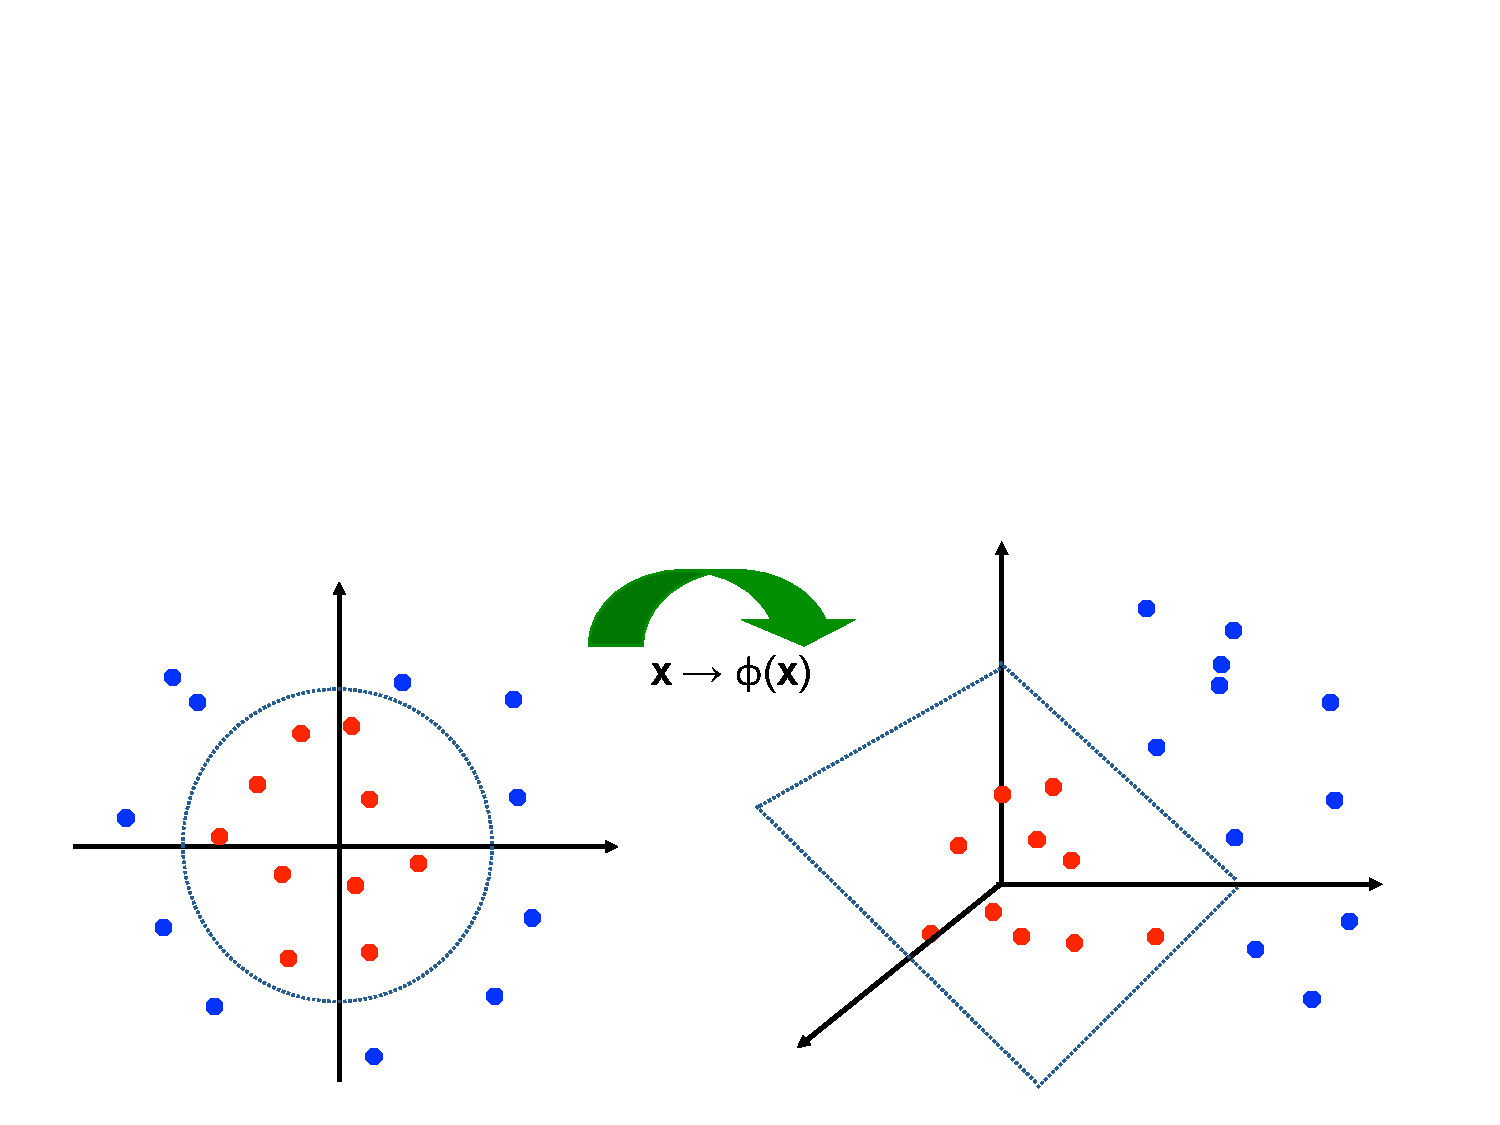
\includegraphics[width=2.5in]{figures/example_kernel_separation.pdf}  \hfill \\

The decision boundary would be a circle.  % wk 8 audio
\hfill \\

If you can't figure out what features you should use, this is a good approach.  % wk 8 audio. 
You don't need the features themselves (??).   \hfill \\
?? You just need the kernel/similarity? matrix.??   \hfill \\
? gram matrix?   \hfill \\


General idea: \hfill \\
If $\bm{x}$ is in $R^n$, then $\phi(\bm{x})$ is in $R^m$ for $m>n$. \hfill \\
We can now learn feature weights $\bm{w}$ in $R^m$ and predict using $y = sign(\bm{w} \cdot \phi(\bm{x}))$. \hfill \\
\hfill \\

\textbf{A linear function in the higher dimensional space will be non-linear in the original space.}  \hfill \\
\hfill \\

% wk 8 audio. 
Say you had a 100,000 points, each of which have a100-dimensional (binary) feature vector.
The chances of being able to find a hyperplane that divides random assignments of binary values is very good.
Almost all of those vertices are empty.
So your chance of finding a desirable hyperplane increases dramatically.  
??? Did I get this right?  Seems like we need to be comparing a feature vector to a transformed feature vector.  
??? 
\hfill \\  \hfill \\

\subsubsection{Danger of Mapping to a Higher Dimensional Space:}
The number of terms in a polynomial of degree $d$ for $m$ input features is 
$\displaystyle {d + m - 1}\choose{d} $ $ \displaystyle = \frac{d + m - 1}{d!(m-1)!}$. \hfill \\
This grows fast!  For $d=6$, $m=100$ you get about 1.6 billion terms.  \hfill \\

We are taking a dot product of $m$ rows for the feature space times $d$ columns of polynomial. 
But you also have terms for combinations of features.  E.g. 
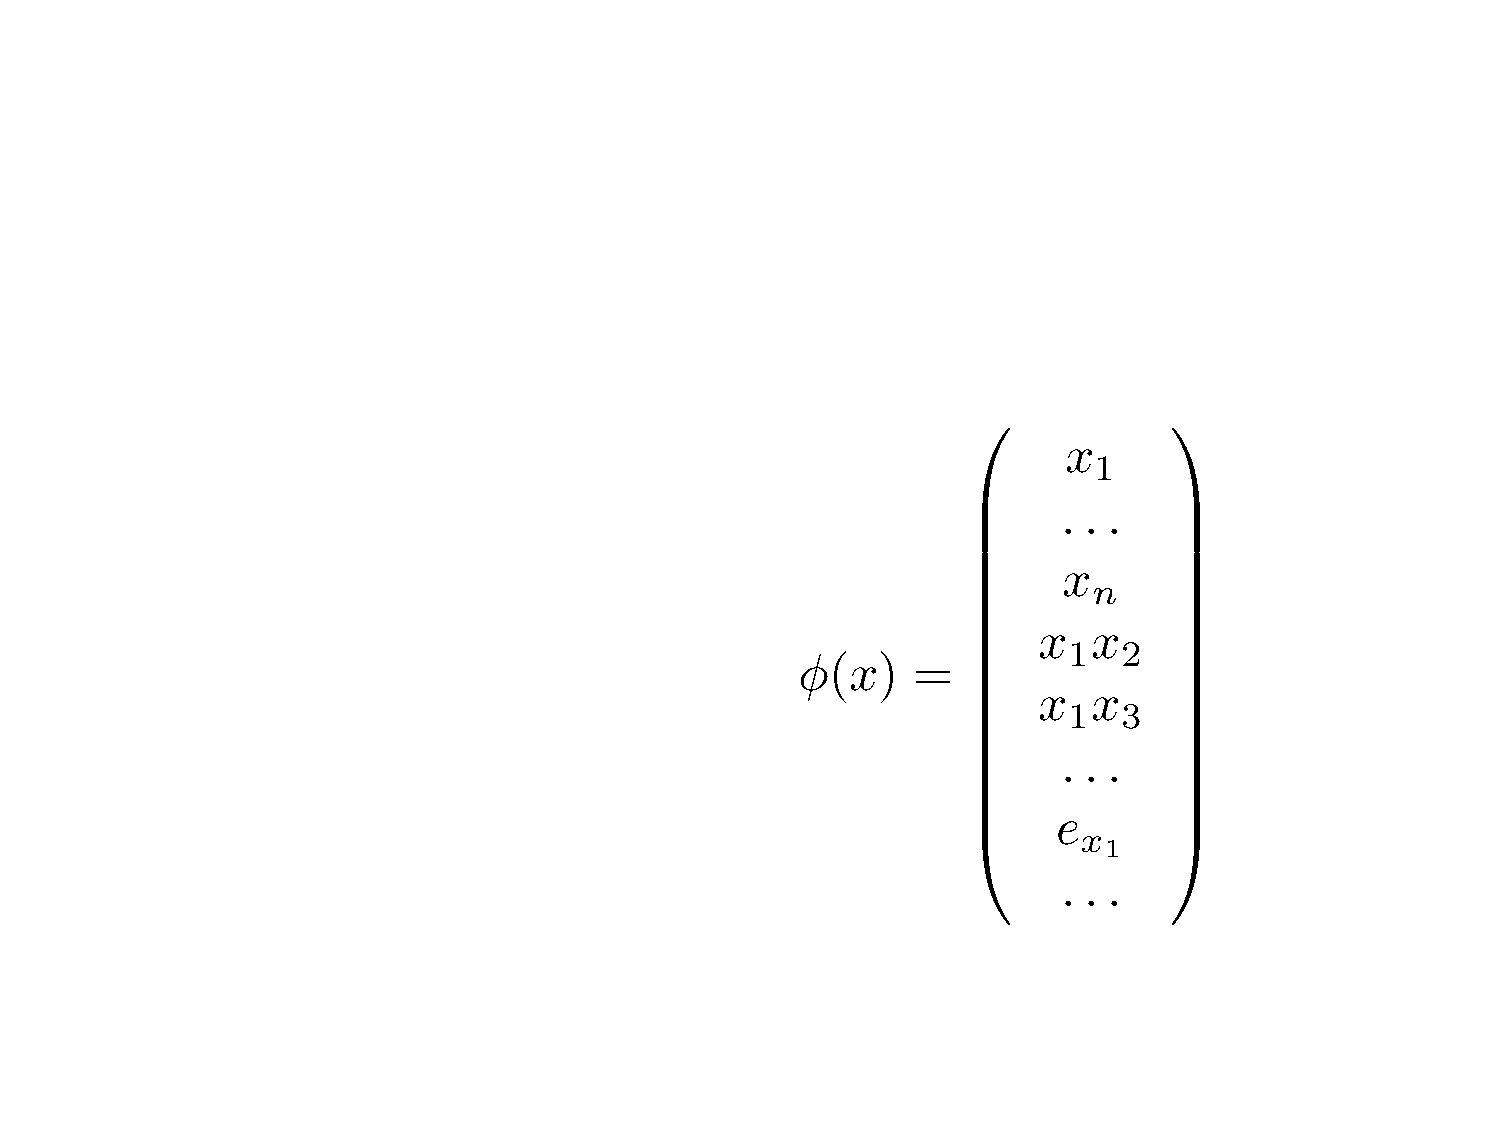
\includegraphics[width=0.8in]{figures/example_kernel.pdf}

\subsubsection{Efficient dot-product of polynomials}
For polynomials of degree exactly $d$, the dot product in higher dimensional space can be written as a dot product in lower dimensional space.  \hfill \\
For $m=2$ (2 features): \hfill \\
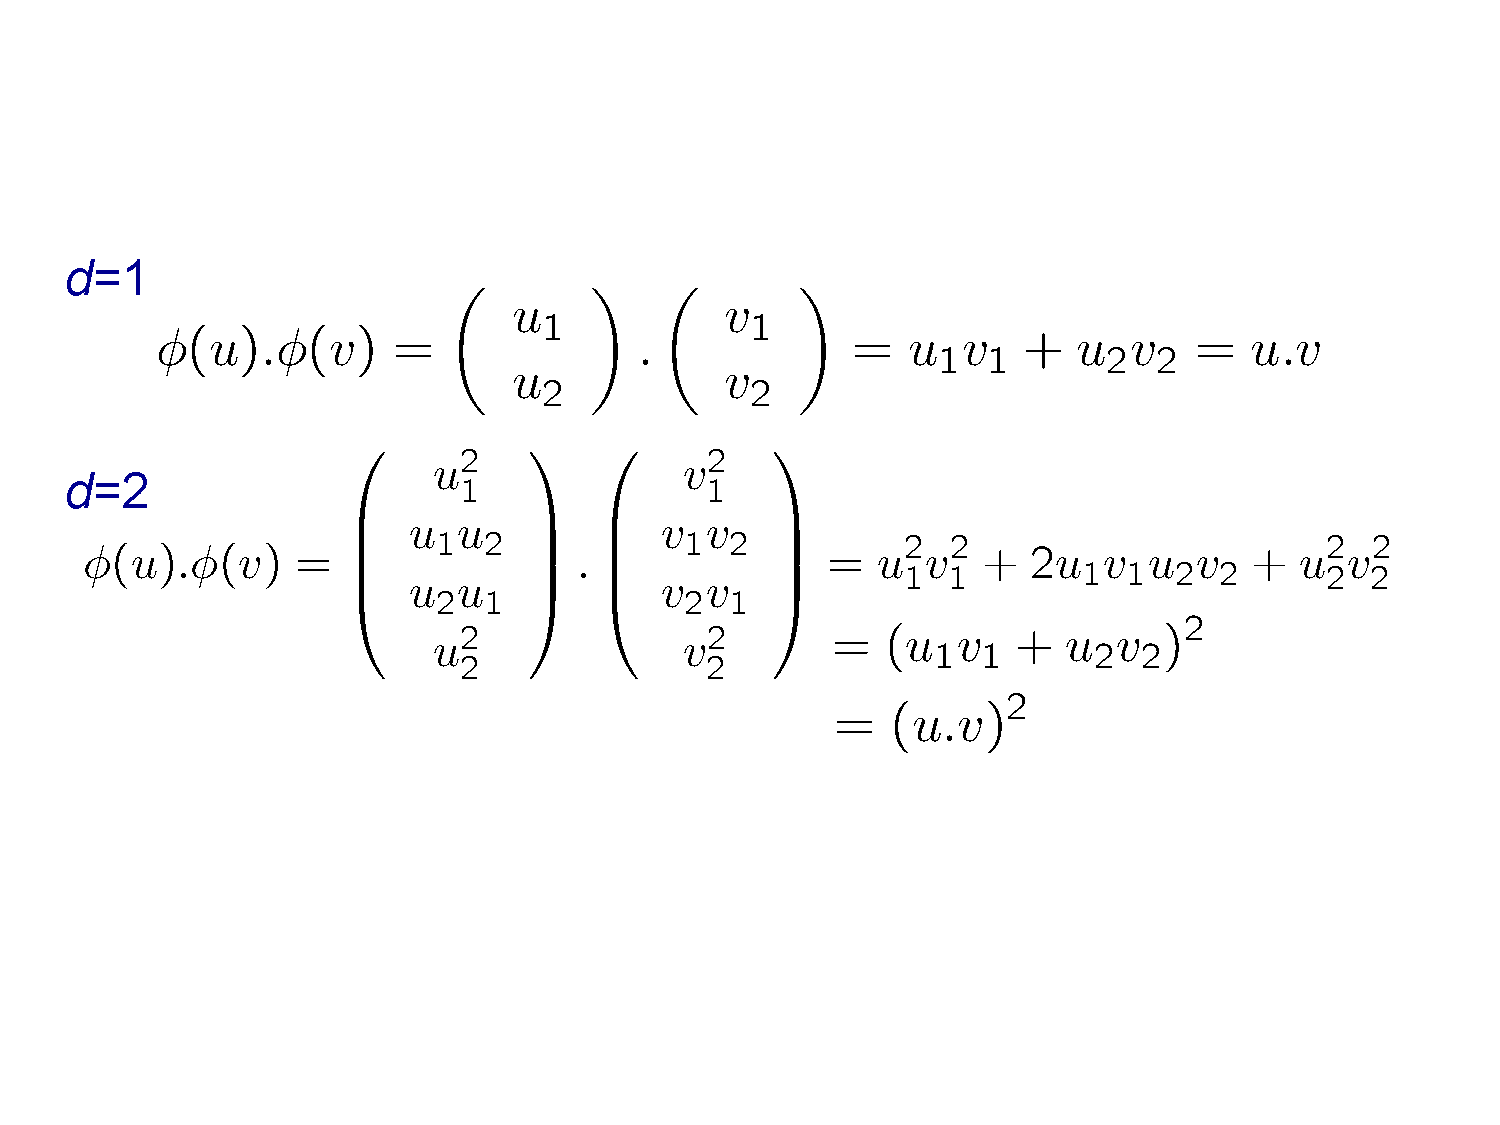
\includegraphics[width=2.5in]{figures/kernel_dot_polynomials.pdf}  \hfill \\
note: here the $.$ is a dot product, not horizontal space fill like a previous lecture. \hfill \\
$u_1$ is feature 1's value, and $u_2$ is feature 2's value. \hfill \\
Polynomial of exactly degree $d$ means we \underline{don't} have a constant bias term like in homework 3 with $[1, \sqrt{2}u, u^2]$  \hfill \\
This is just factoring.  \hfill \\
\hfill \\

Proof not shown, but for any $d$: \hfill \\
$K(u, v) = \bm{\phi}(u).\bm{\phi}(v) = (u.v)^d$

\subsection{The "Kernel Trick"}

We like the idea of going to higher dim, but we don't like the idea of operating in it.  Expensive. \hfill \\
\hfill \\

With this trick, we won't ever compute a dot product in the expensive space.   % wk 8 audio
Not all $\phi$ satisfy, but there are big categories that do it.  % wk 8 audio
Need to be able to represent a higher dim space as one in a lower dim space.  % wk 8 audio
Usually exponentiation is used.  %wk 8 audio. 
%But it doesn't work with all projections, .  Just special ones. 
\hfill \\ \hfill \\

A \textbf{kernel function} defines a dot product in some feature space: 
\begin{align*}
	K(\bm{u}, \bm{v}) =\bm{\phi}(\bm{u}) \cdot \bm{\phi}(\bm{v})
\end{align*}
Where $\bm{u}$, $\bm{v}$ are points in your training or test set, each with their own features. \hfill \\ 
Or $\bm{u}$ could be a data point and $\bm{v}$ could be the $\bm{w}$ of the hyperplane that you need to dot against to classify new points.
 \hfill \\
 
 If $\bm{u}$, $\bm{v}$ each have two dimensions (2 features): \hfill \\

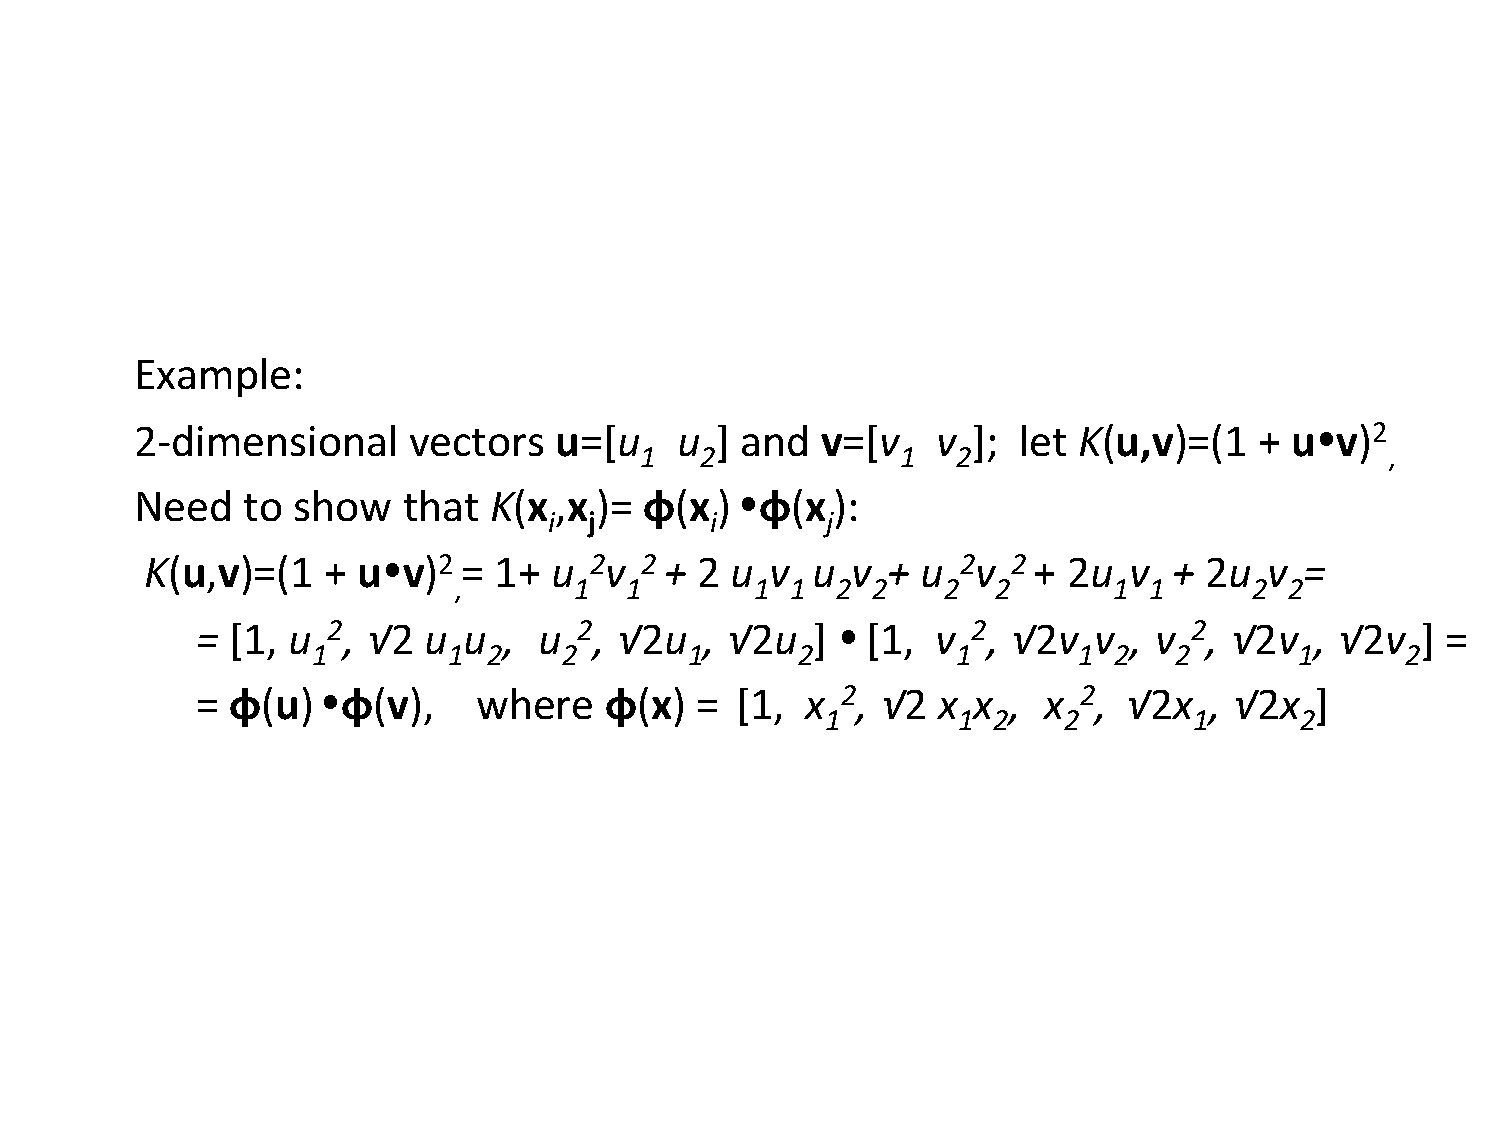
\includegraphics[width=3.1in]{figures/example_kernel_math.pdf} \hfill \\
Thus, a kernel function \textit{implicitly} maps data to a high-dimensional space without the need to compute each $\bm{\phi}(\bm{x})$ explicitly.   \hfill \\
If we had $d = 100$ instead, our savings would be huge. 
 \hfill \\

Translation for this particular kernel: \hfill \\
We want to get the perks of the high dimensional space given by $\bm{\phi}(\bm{x}) = [1, x_1^2, \sqrt{2}x_1 x_2, x_2^2, \sqrt{2} x_1, \sqrt{2} x_2]$ where $\bm{x}$ is either $\bm{u}$ or $\bm{v}$.  \hfill \\
But this is computationally expensive because there are many terms in that thing.  \hfill \\
If we take the dot product of two vectors $\bm{\phi}(\bm{u})$, $\bm{\phi}(\bm{v})$ we get some magic: \hfill \\
\begin{align*}
	\bm{\phi}(\bm{u}) \cdot \bm{\phi}(\bm{v}) &= [1, u_1^2, \sqrt{2}u_1 u_2, u_2^2, \sqrt{2} u_1, \sqrt{2} u_2]  \cdot \quad \mbox{(line wrapped)} \\
			& \quad \quad [1, v_1^2, \sqrt{2}v_1 v_2, v_2^2, \sqrt{2} v_1, \sqrt{2} v_2]   \\
		&=  (1 + \bm{u} \cdot \bm{v})^2
\end{align*}
Can do $(1 + \bm{u} \cdot \bm{v})^2$ with a dot product that only includes multiplying $[u_1, u_2]^T[v_1, v_2]$.     \hfill \\ 
That's a lot less computation/memory expensive than the full dot product above.  \hfill \\
If that leads to good separation, you are a happy machine learner!   \hfill \\
\textbf{This is true for other kernels in general.}   \hfill \\
($(1 + \bm{u} \cdot \bm{v})^2$ would take other forms for other cases).   \hfill \\
\hfill \\

It is essential that everything you want to do with your transformed vectors is representable by simple dot products.
If you can't simplify it down to dot products of the original vector then there's no point. 

\subsection{"Kernel Trick" for the Perceptron}

\subsubsection{Intro to $ \displaystyle w = \sum_k a^k \phi(x^k)$}
If we wanted to apply a transformation of the data $\phi(x^i)$ to each of our $x^i$ training points, we would do: \hfill \\
For $t = 1 \dots T$, $i = 1, \dots n$:
\begin{itemize}
	\item $ y = sign(w \cdot \phi(x^i))$
	\item if $y \neq y^i$:  (if class wasn't predicted correctly)
	\begin{itemize}
		\item $ \quad w = w + y^i \phi(x^i)$  % update $w$: 
		%\item $a^i += y^i$
	\end{itemize}
\end{itemize}

We can re-write $w$ as $ \displaystyle \sum_j y^j x^j$ for one loop over the data, if $j$ is the index of the points that were wrongly classified and thus contributed to the weights $w$.  
but we have multiple epochs: $t = 1 \dots T$.  
The point might be classified wrong the first time but right the 2nd and 3rd times.  \hfill \\
So we can use different notation to keep track of how each point adds to the weights
	depending on whether it was predicted correctly and whether it was a $y=1$ or $y = -1$.  \hfill \\
	
This looks like $ \displaystyle w = \sum_k a^k \phi(x^k)$   \hfill \\
We get $a^k$ from the modified loop over the data points shown below. \hfill \\
Note: we switch from index $i$ over the data points to $k$ because we might see data points that are identical in the training set.  
We don't need to keep track of those $\phi(x^k)$ points separately with separate $k$ indices and hence $a^k$ values if they are the same.  
Just keep summing up their signs as needed to modify $w$. 

New protocol: \hfill \\
For $t = 1 \dots T$, $i = 1, \dots n$:
\begin{itemize}
	\item $ y = sign(w \cdot \phi(x^i)$
	\item if $y \neq y^i$:  (if class wasn't predicted correctly)
	\begin{itemize}
		%\item $ \quad w = w + y^i \phi(x^i)$  % update $w$: 
		\item $ \quad a^i += y^i$
	\end{itemize}
\end{itemize}

For example, say you loop over data point $k$ with $\phi(x^k) = [1, 2, 3]$ and label $y^k = -1$ three times.
If you got it wrong the first two times and right the third time you would have this point contributing 
$w = -[1, 2, 3] -[1, 2, 3] + 0[1, 2, 3]$. \hfill \\
In the loop we would have had $a^k = -1 -1$ for the two passes through that we got it wrong.  \hfill \\

If we kept track of those $a$ values for all $i$ or $k$ data points, then we get that thing above: 
$ \displaystyle w = \sum_k a^k \phi(x^k)$ 

\subsubsection{The Kernelized Perceptron} % $w = \sum_k a^k \phi(x^k)$ in 

Protocol: \hfill \\
Set $a^i = 0$ for each example $i$ \hfill \\
For $t = 1 \dots T$, $i = 1, \dots n$:  \hfill \\
\begin{itemize}
	\item $ \displaystyle y = w \cdot \phi(x^i) $ \hfill \\
			 $ \displaystyle \quad \mbox{use } w = \sum_k a^k \phi(x^k) $  \hfill \\
			$ \displaystyle \quad = sign( ( \sum_k a^k \phi(x^k))  \cdot \phi(x^i))$  \hfill \\
			$ \displaystyle  \quad = sign( \sum_k a^k K(x^k, x^i) )$
	\item if $y \neq y^i$:  (if class wasn't predicted correctly)
	\begin{itemize}
		%\item $ \quad w = w + y^i \phi(x^i)$  % update $w$: 
		\item $ \quad a^i += y^i$
	\end{itemize}
\end{itemize}

The points: 
\begin{itemize}
	\item We never compute the features explicitly. \hfill \\
		If $x^i$ has 3 features, $\phi(x^i)$ might have 9 items such as polynomials.  \hfill \\
		But we don't have to calculate those 9 features if they correspond to a Kernel. \hfill \\
		We might be able to use something like the simplification to $(1 + \bm{u} \cdot \bm{v})^2$ 
			simplification just before this. 
	\item We compute the dot products in "closed form": $K(u, v) = \phi(u) \cdot \phi(v)$ \hfill \\
		A "closed form" expression is a mathematical expression that can 
			be evaluated in a finite number of operations.
		(You can calculate it efficiently; it is possible you would have an infinite number of features.)  % Erick 2/24 
 
\hfill \\

\end{itemize}

\subsubsection{Kernelized Perceptron Example}

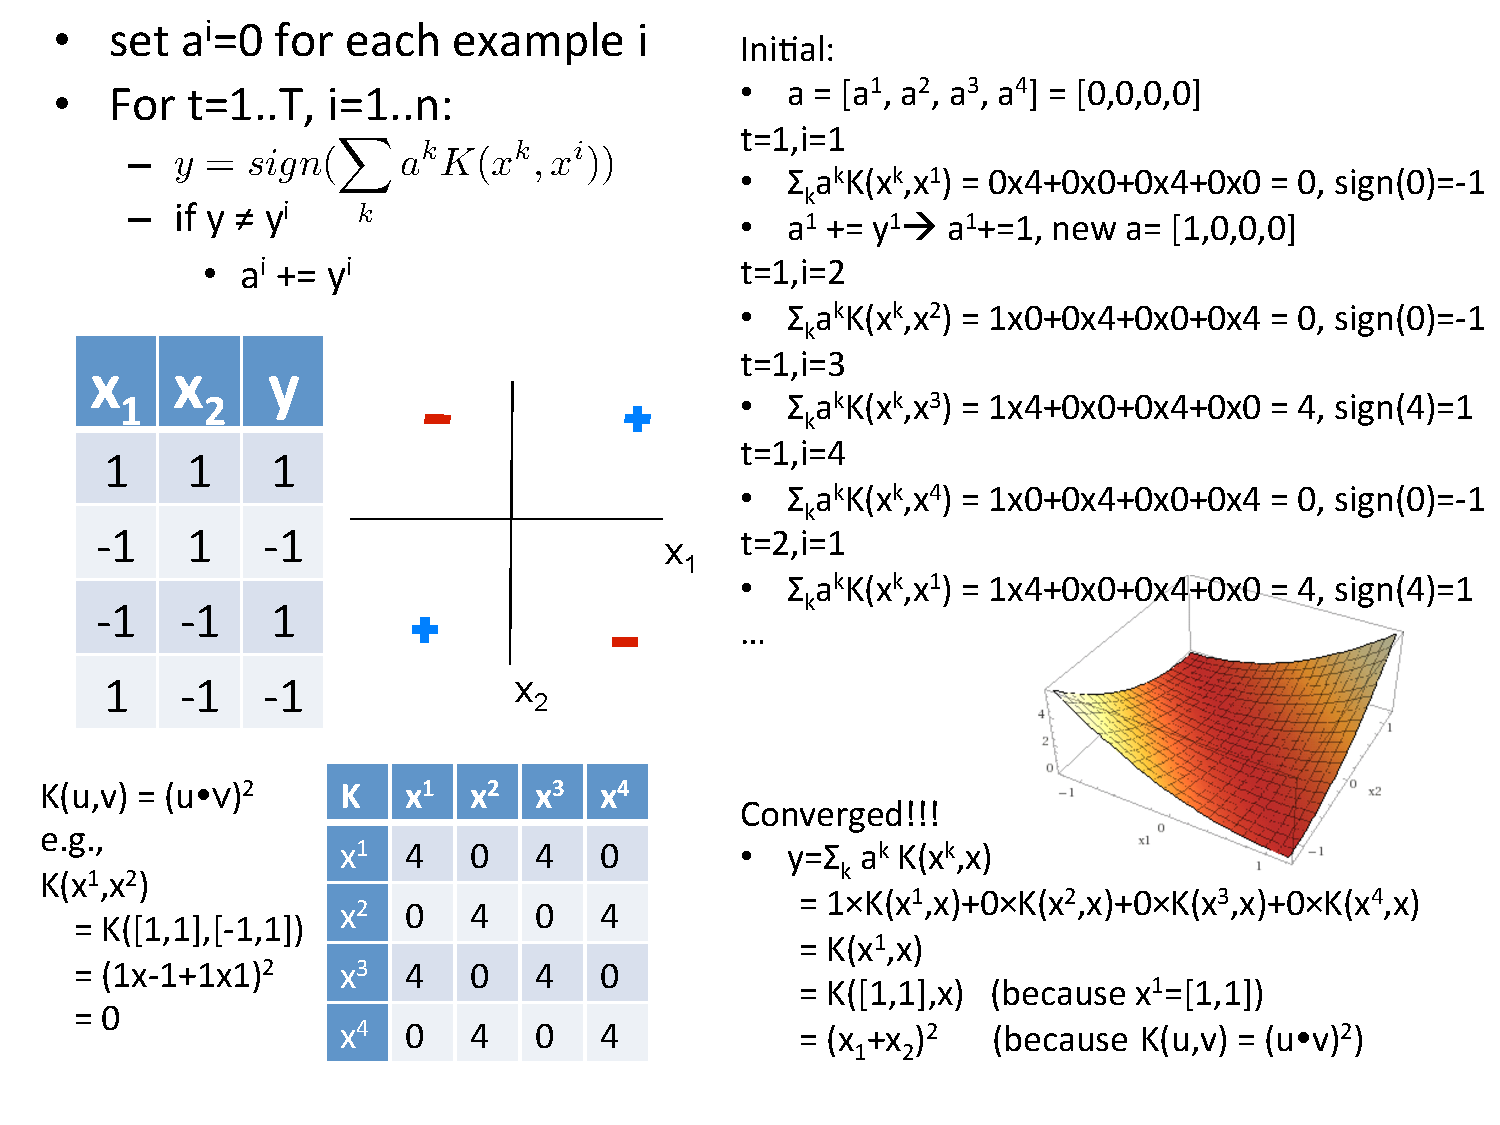
\includegraphics[width=3.4in]{figures/kernelized_perceptron_example.pdf}

\subsubsection{Common Kernels}

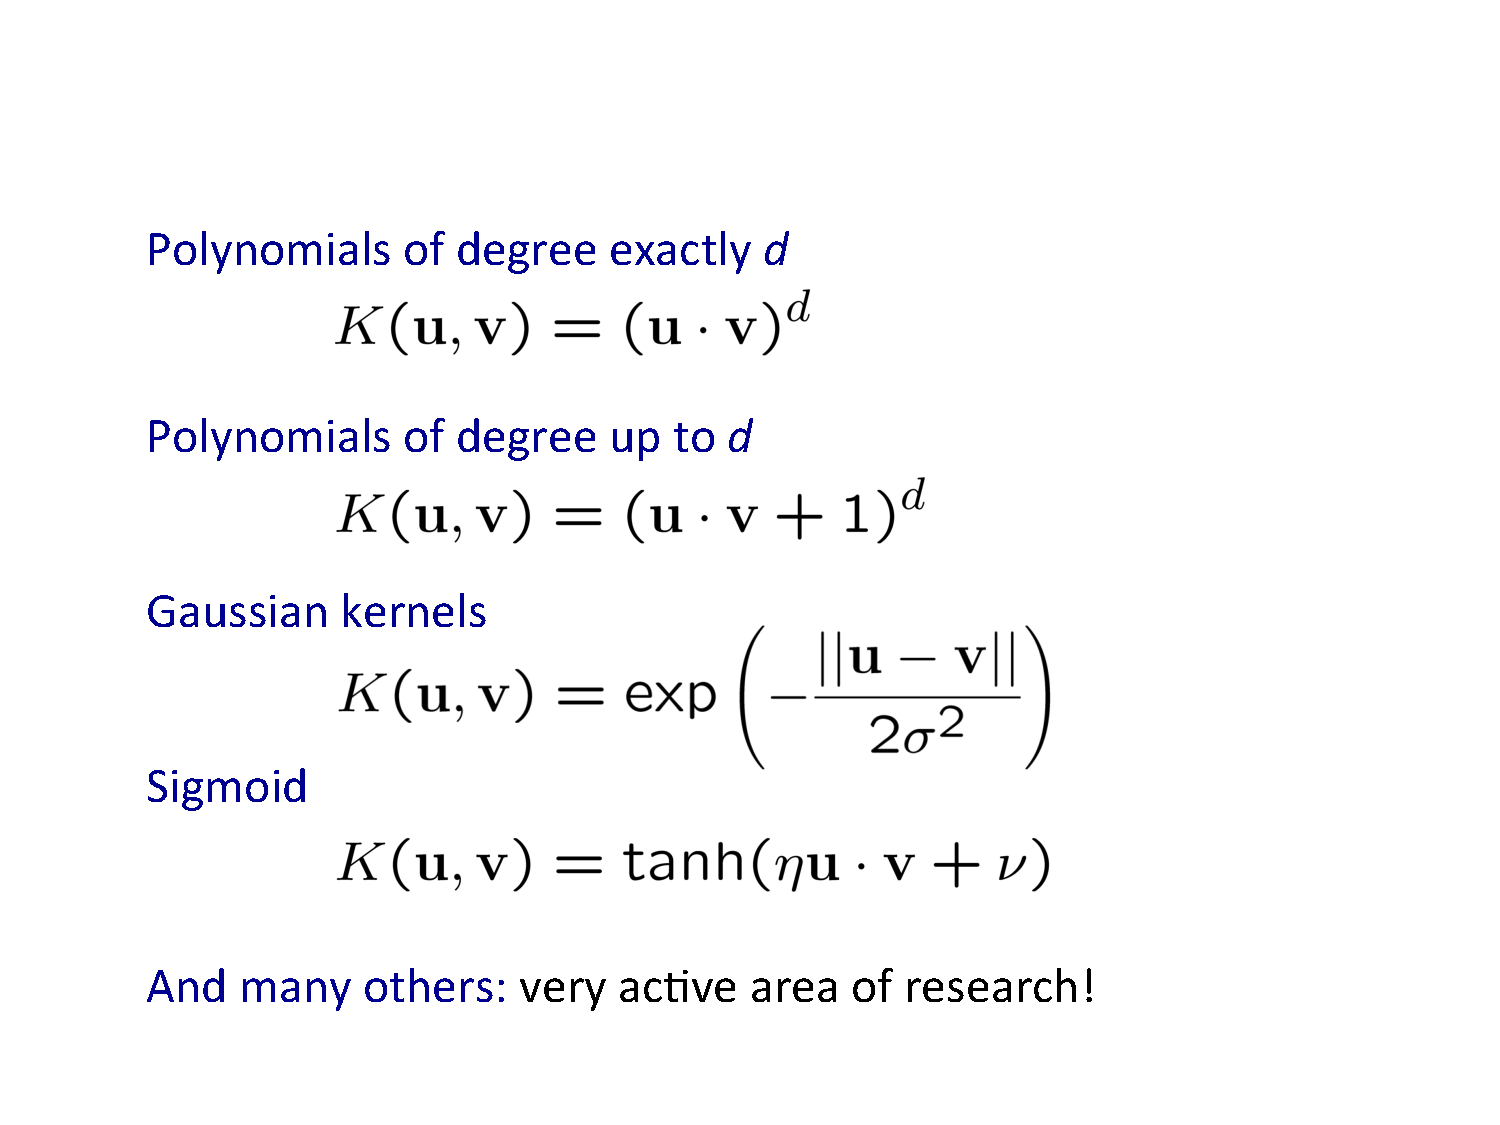
\includegraphics[width=2.0in]{figures/common_kernels.pdf}

\subsubsection{Kernels: Overfitting}

With Kernels we have a huge feature space, so over-fitting can happen. \hfill \\
It turns out, however, that it can be robust to overfitting. \hfill \\
Can do things like limiting the number of updates the Perceptron does. \hfill \\
SVMs have have a clearer story for avoiding overfitting.  \hfill \\

Do keep in mind that \textbf{everything overfits sometimes}!

You can also control by:
\begin{itemize}
	\item Choosing a better Kernel
	\item Varying parameters of the Kernel, such as the width of Gaussian.
\end{itemize}

\subsubsection{Kernels in Logistic Regression}
Had: \hfill \\
$P(Y=0 | \bm{X}= \bm{x}, \bm{w}, w_0 )= \frac{1}{1 + \exp(w_0 + \bm{w}\cdot \bm{x})}$ \hfill \\
 \hfill \\

We can define weights in terms of data points: \hfill \\
$\displaystyle  \bm{w} = \sum_j \alpha^j \phi(\bm{x}^j)$  \hfill \\
That leads to 
\begin{align*}
	P(Y=0 | \bm{X}= \bm{x}, \bm{w}, w_0 ) &= \frac{1}{1 + \exp(w_0 +  \sum_j  \alpha^j \phi(\bm{x}^j) \cdot \phi(\bm{x}))} \\
		& = \frac{1}{1 + \exp(w_0 +  \sum_j  \alpha^j K(\bm{x}^j , \bm{x})} \\
\end{align*}

We can derive the gradient descent rule on $\alpha^j$, $w_0$.  ???  \hfill \\

Similar tricks for all linear models: SVMs, etc. 


